\section{Project planning}
\subsection{Schedule}

\subsubsection{Estimated duration}
The work required for this project, including development, documentation, possible bugs and fixes, is approximately 4 months.

All possible issues mentioned in deliverable 1 are taken into account when designing this planning. However, during project development it might be possible that the proposed planning is altered.

\subsection{Task description}

This project has a lot of different modules that are independent from each other in functionality, but some might require the output of a previous module before being able to work properly. The planning is important to follow, so we do not break time dependencies between the modules.

\subsubsection{Initial 3D Viewer and GUI}
We will use \emph{three.js} as a base for the 3D viewer and will work on top of it. It's fairly easy to set up and show any 3D model in the viewer, as it's one of the basic examples included in the library. We then need some functions to rotate, scale, translate and otherwise manipulate the object. I have some experience with three.js, so this task should last no longer than a week. This task requires the use of the mentioned library, as well as an IDE. We will use WebStorm \cite{webstorm} for the development of the project and all of it's components.

\subsubsection{Slicer}
Sharing the name with the overall process, in this case the slicing algorithm will only be responsible for obtaining a polygon for a given height. This module will be called multiple times in order to slice the whole object.

\subsubsection{Toolpath generator}
After the slicer has generated a polygon, this module will be responsible for generating a set of lines in an internal format that will be used by the \emph{GCODE} generator later on.

\subsubsection{GCODE generator}
Once we have our toolpath generated, we need to convert it to a language the 3D Printer understands: GCODE. This module is responsible for the conversion and the final output of the program. This task requires a 3D printer or simulator to test the generated output.



\subsubsection{Resources}

The following resources are required in order to complete the previous tasks.

\begin{itemize}
    \item All modules require \emph{human resources} to develop the required code.
    \item A computer to develop with.
    \item A 3D printer or simulator to test the output of the slicer.
    \item A place for the developer to work
    \item All the mentioned software
\end{itemize}


\subsection{Time estimation}
An estimation of the project's timeline is shown in \autoref{table:task-time}. Times are approximate but should account for most possible changes and delays.

\FloatBarrier
\begin{table}[h!]
\centering
\begin{tabular}{ |c|c| } 
    \hline
    Task & Estimated duration (h)  \\ 
    \hline
    
    \hline
    GEP & 75  \\ 
    \hline
    Project setup & 20  \\ 
    \hline
    3D Viewer & 40  \\ 
    \hline
    GUI & 25  \\ 
    \hline
    Slicer & 80  \\ 
    \hline
    Toolpath generator & 80  \\ 
    \hline
    GCODE generator & 80  \\ 
    \hline
    Bugfixes and improvements & 50 \\
    
    \hline
    Total & 450 \\
    \hline
\end{tabular}
\caption{Estimated time for each task}\label{table:task-time}
\end{table}
\FloatBarrier


Every task or module will have several stages. We will need to read through existing examples and projects to get a general idea of what to do. Then we will need to decide the implementation details, implement the module, test it and fix any possible bugs.

\subsubsection{Gantt chart}

\autoref{fig:gantt-chart} shows a more detailed overview of the task planning in a Gantt chart. The timeline may change slightly due to project requirements or unexpected bugs. This is accounted for in the final stage of the project, bugfixes and improvements. More on this in the next section.


\begin{figure}[H]
    \noindent\makebox[\textwidth]{
        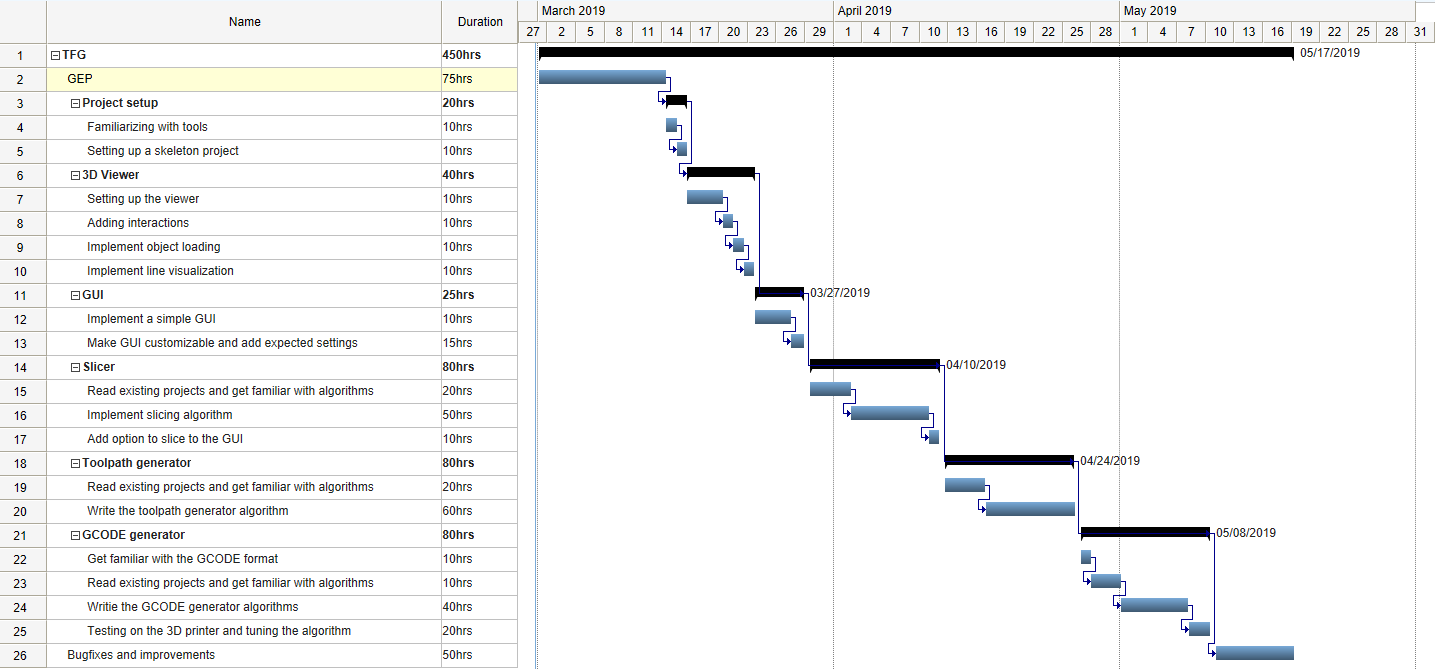
\includegraphics[width=1.3\textwidth]{images/gantt.png}
    }
    \caption{Gantt chart of the project. Generated with Gantter \cite{gantter}}
    \label{fig:gantt-chart}
\end{figure}


\subsection{Alternatives and action plan}

In the previous delivery we mentioned the methodologies that will be used, including Test Driven Development, and heavy use of git. This should reduce the risk of bugs and accelerate the development quality as well as the speed.

We have a total workload of 450 hours, with a dedication 40 hours per week. Extra time is given at the end to account for possible bugs or potential problems and slowdowns, which are discussed in the previous delivery.

The 50 hours of bug fixes and improvements are not necessarily at the end. Instead they are distributed throughout the project. In case of a problem, the complete focus will be on solving it as soon as possible, and this time will be deducted from the bug fix time at the end. Any time left at the end will be used for improvements.

Particular detailed are discussed as follows:

\subsubsection{Breaking the 3D printer}
We will mitigate the risk of breaking the 3D printer by running wrong gcode on it by simulating it first. Slic3r and Cura both have a gcode viewer, so we can verify that the generated output is correct (or at least it won't move to negative coordinates, or outside of the build area). In case the printer ends up breaking, we have an alternative, cheaper 3D printer available for testing.

\subsubsection{Floating point precision}
Floating point precision may not be enough for some geometry operations. In these rare cases, the model will still be sliced correctly, but will have some features or some missing detail. This is a limitation of all slicers, and it is possible to still get those detail, but no current slicer does this so we consider this beyond the scope of this project.

\subsubsection{Bugs}
We already discussed multiple times how we will deal with possible bugs. In particular, whenever a bug is found, we will write a test case that reproduces the bug, and use git bisect to find the exact commit where the bug was introduced. Since we are also making small commits with specific changes, it will be easy to find out what the cause of the bug was and how to fix it.

\subsubsection{Algorithm efficiency}
Some of the slowest algorithms are already handled by libraries, but we still need to find efficient algorithms for slicing, polygon generation and toolpath generation. We have assigned extra time to each of these module's planned time to account for finding efficiency improvements. Since most slicers are able to run on slow hardware, it is very likely that every algorithm will be possible to implement with acceptable efficiency. Alternatively we can accept slower algorithms that will still produce a decent running time, although it will be noticeable to the user.
